% Chapter 3

\chapter{Methodology} % Main chapter title

\label{Chapter3} % For referencing the chapter elsewhere, use \ref{Chapter1} 

\lhead{Chapter 3. \emph{Methodology}} % This is for the header on each page - perhaps a shortened title

%----------------------------------------------------------------------------------------
\section{Data Collection and Quality}
The data used in this study was freely collected from the Yahoo finance web site (www.yahoo.com). It is of high quality with no missing values and represents the opening, high, low and closing prices for each day that the particular market indice was open for trading. 

\section{Data Description}
Data from a variety of national stock market indices was employed in this study. The indices were from a variety of geographic locations with FTSE (UK), DAX (Germany) and CAC (France) all being in Europe, the Dow is from the US, the Nikkei from Japan and AORD from Australia. The data is in the form of so-called daily OHLC (daily open, high, low and close prices) for Monday to Friday (excluding appropriate national holidays) for the period 2000 until the end of 2013. A schematic representation of daily OHLC data can be seen in Figure \ref{fig:chp3_ohlc}. The first six observations from the DAX data set (German national indice) can be seen in Table \ref{tab:daxhead}.

%------------------- Graph of OHLC ---------------------------------
\begin{figure}[tbh]
\centering
%\includegraphics[width=6cm]{../Figures/chp3_ohlc}
\includegraphics[width=6cm]{chp3_ohlc}
\caption[Open, high, low and closing prices (OHLC).]{A schematic representation of open, high, low and closing prices (OHLC).}
\label{fig:chp3_ohlc}
\end{figure}

The final six observations from the DAX data set can be seen in Table \ref{tab:daxtail}. Over the period of the data (2000 until the end of 2013) the DAX started at 6691 and finished at 9552. Summary statistics for the DAX data set can be seen in Table \ref{tab:daxsum}. The data set contains 3621 observations and the closing price has ranged between 2202 and 9742 over the period. A graph of the closing prices from 2000 to 2013 and be seen in Figure \ref{fig:Dax2000_2013} and a graph for 2013 can be seen in Figure \ref{fig:Dax2013}.

%------------------- Table of 1st 6 rows of DAX ---------------------------------


%label - tab:daxhead
% latex table generated in R 3.1.0 by xtable 1.7-3 package
% Wed May 28 17:43:16 2014
\begin{table}[ht]
\centering
\caption[First 6 rows of the Dax data set.]{First 6 rows of the Dax data set} 
\label{tab:daxhead}
\begin{tabular}{lcccc}
  \toprule Date & Open & High & Low & Close \\ 
  \midrule 03/01/2000 & 6962 & 7159 & 6721 & 6751 \\ 
  04/01/2000 & 6747 & 6755 & 6510 & 6587 \\ 
  05/01/2000 & 6586 & 6586 & 6389 & 6502 \\ 
  06/01/2000 & 6501 & 6539 & 6403 & 6475 \\ 
  07/01/2000 & 6490 & 6792 & 6470 & 6781 \\ 
  10/01/2000 & 6785 & 6975 & 6785 & 6926 \\ 
   \bottomrule \end{tabular}
\end{table}


%\begin{table}[!htbp] \centering	
%\caption[Dax table set - head.]{First six rows of the Dax data set.}
%\label{tab:daxhead}
%\begin{tabular}{lcccc}
%\toprule
%Date & Open & High & Low & Close \\
%\midrule
%03/01/2000 & $6,961.72$ & $7,159.33$ & $6,720.87$ & $6,750.7$ \\
%04/01/2000 & $6,747.24$ & $6,755.36$ & $6,510.46$ & $6,586.95$ \\
%05/01/2000 & $6,585.85$ & $6,585.85$ & $6,388.91$ & $6,502.07$ \\
%06/01/2000 & $6,501.45$ & $6,539.31$ & $6,402.63$ & $6,474.92$ \\
%07/01/2000 & $6,489.94$ & $6,791.53$ & $6,470.14$ & $6,780.96$ \\
%10/01/2000 & $6,785.47$ & $6,975.26$ & $6,785.47$ & $6,925.52$ \\
%\bottomrule
%%\normalsize
%\end{tabular}
%\end{table}


%label - tab:daxtail
% latex table generated in R 3.1.0 by xtable 1.7-3 package
% Wed May 28 17:41:24 2014
\begin{table}[ht]
\centering
\caption[Final 6 rows of the Dax data set.]{Final 6 rows of the Dax data set} 
\label{tab:daxtail}
\begin{tabular}{lcccc}
  \toprule Date & Open & High & Low & Close \\ 
  \midrule 13/12/2013 & 9017 & 9047 & 8991 & 9006 \\ 
  16/12/2013 & 9005 & 9188 & 8998 & 9164 \\ 
  17/12/2013 & 9143 & 9162 & 9085 & 9085 \\ 
  18/12/2013 & 9145 & 9191 & 9122 & 9182 \\ 
  19/12/2013 & 9280 & 9352 & 9257 & 9336 \\ 
  20/12/2013 & 9371 & 9413 & 9353 & 9400 \\ 
   \bottomrule \end{tabular}
\end{table}


% latex table generated in R 3.0.2 by xtable 1.7-1 package
% Sat Apr 12 12:45:35 2014
%\begin{table}[ht]
%\centering
%\caption[Dax table set - tail.]{Final six rows of the Dax data set.}
%\label{tab:daxtail}
%\begin{tabular}{lrrrr}
%  \toprule
% Date & Open & High & Low & Close \\ 
%  \midrule
%  18/12/2013 & 9145.35 & 9190.73 & 9122.05 & 9181.75 \\ 
%  19/12/2013 & 9279.68 & 9351.90 & 9257.24 & 9335.74 \\ 
%  20/12/2013 & 9371.08 & 9413.09 & 9352.98 & 9400.18 \\ 
%  23/12/2013 & 9436.49 & 9488.82 & 9427.54 & 9488.82 \\ 
%  27/12/2013 & 9558.55 & 9589.39 & 9548.89 & 9589.39 \\ 
%  30/12/2013 & 9586.53 & 9594.35 & 9552.16 & 9552.16 \\ 
%  \bottomrule
%\end{tabular} 
%\end{table}

% tabularx version ...
%\begin{table}[!htbp] \centering
%\caption[Dax table set.]{First six rows of the Dax data set.}
%\label{tab:dax2}
%\begin{tabularx}{\textwidth}{l >{\centering}X >{\centering}X >{\centering}X X<{\centering}}
%  \toprule
%  Date & Open & High & Low & Close \\
% \midrule
%03/01/2000 & $6,961.720$ & $7,159.330$ & $6,720.870$ & $6,750.760$ \\
%04/01/2000 & $6,747.240$ & $6,755.360$ & $6,510.460$ & $6,586.950$ \\
%05/01/2000 & $6,585.850$ & $6,585.850$ & $6,388.910$ & $6,502.070$ \\
%06/01/2000 & $6,501.450$ & $6,539.310$ & $6,402.630$ & $6,474.920$ \\
%07/01/2000 & $6,489.940$ & $6,791.530$ & $6,470.140$ & $6,780.960$ \\
%10/01/2000 & $6,785.470$ & $6,975.260$ & $6,785.470$ & $6,925.520$ \\
%  \bottomrule
%\end{tabularx}
%\end{table}



% ------ Table of Summary stats of Dax --------------
\begin{table}[!htbp] \centering
\caption[DAX summary statistics]{Summary statistics of the DAX data set.}
\label{tab:daxsum}
\begin{tabular}{lccccc}
\toprule
Statistic & N & Mean & St. Dev & Min & Max \\
\midrule
Open  & 3,621 & 5,858.36 & 1,559.40 & 2,203.97 & 9,752.11 \\
High  & 3,621 & 5,906.70 & 1,561.17 & 2,319.65 & 9,794.05 \\
Low   & 3,621 & 5,804.85 & 1,557.49 & 2,188.75 & 9,714.02 \\
Close & 3,621 & 5,857.74 & 1,559.39 & 2,202.96 & 9,742.96 \\
\bottomrule
%\normalsize
\end{tabular}
\end{table}


% ------ Graph of DAX 2000 to 2013 --------------
\begin{figure}[tbph]
\centering
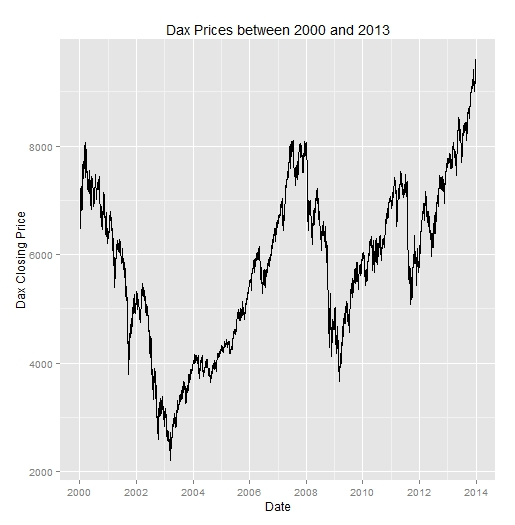
\includegraphics[width=9cm]{chp3_Dax2000_2013}
\caption[Graph of DAX between 2000 and 2013]{Graph of German DAX between 2000 and 2013.}
\label{fig:Dax2000_2013}
\end{figure}

% ------ Graph of Dax 2000 to 2013 --------------
\begin{figure}[tbph]
\centering
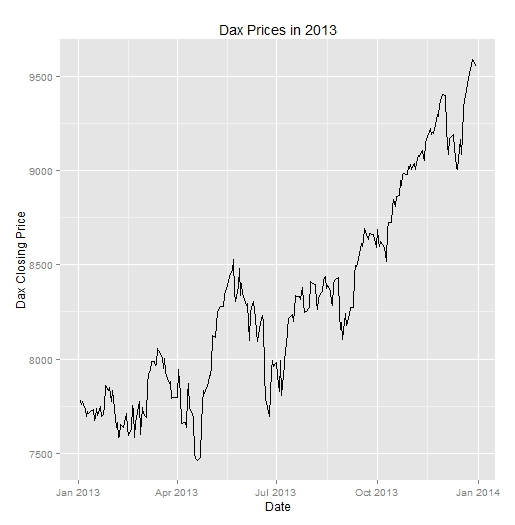
\includegraphics[width=9cm]{chp3_Dax_2013}
\caption[Graph of DAX in 2013]{Graph of German DAX in 2013.}
\label{fig:Dax2013}
\end{figure}

Each data set has a particular set of characteristics and these are important when technical analysis and other analytical techniques are applied to the data set \citep{Chen201466,Matheson2012441}. A variety of these are explored in the following sections. The average amount a market moves is investigated and the term Average True Range is introduced and defined for the data sets. Where the opening and closing prices are in relation to the previous day's high and low values are also considered. Finally, the distance between the day's opening and high prices and opening to low prices are investigated. The relative ratios of these values are important when considering which technical analysis may be best suited to a particular market.

\subsection{Average True Range (ATR)}
\label{chp3:atr}
\cite{wilder1978new} introduced the concept of Average True Range (ATR) as a way to measure a market's volatility or the amount the price is likely to move in any one day. Initially the True Range (TR) is calculated as the maximum of:
\begin{enumerate}
\item the today's high price minus today's low price.
\item the absolute value of the today's high minus the previous day's closing price.
\item the absolute value of the today's low minus the previous day's closing price.
\end{enumerate}
Having calculated the TR, an average of a previous number of days is used to derive the ATR. Typically the TR values from the previous 14 days are used.

Absolute values are used in the calculation of the ATR as we are not concerned with the market direction but rather the the amount the market is likely to move. ATRs are typically quoted as absolute values and as such markets trading at higher prices will have higher ATRs. For example the Japanese Nikkei with a value of 14000 will move more in a day than the French CAC with a value in the 4000's. 

Dividing the ATR by the closing price is a useful way to see how a security's volatility varies over time. Table \ref{tab:atr_dax} shows summary statistics for the ATR and ATR divided by closing price and Figure \ref{fig:Dax_atr} is a graph of how ATR divided by closing price has varied for the DAX between 2000 and 2013. In absolute terms the ATR varied between 36 and 316, however the value of the indice itself varied a lot. Looking at the ATR value divided by the closing period it can be seen that over the period of 2000 to 2014 the mean value is approximately 2. Thus on average the market can be expected to move 2\% of the closing price in any one day. However this value has varied between 0.7\% in periods of low volatility to a value of 6.7\%.

% Table created by stargazer v.4.5.3 by Marek Hlavac, Harvard University. E-mail: hlavac at fas.harvard.edu
% Date and time: Mon, Mar 24, 2014 - 21:57:13
\begin{table}[!htbp] \centering 
  \caption[Average True Range of DAX]{ATR and ATR divided by closing price for the DAX between 2000 and 2013} 
  \label{tab:atr_dax} 
\begin{tabular}{lccccc} 
\toprule
Statistic & N & Mean & St. Dev & Min & Max \\ 
\midrule
ATR & 3,556 & 108.29 & 45.53 & 36.07 & 316.04 \\ 
ATR/Close & 3,556 & 1.995 & 1.065 & 0.700 & 6.740 \\ 
\bottomrule
%\normalsize 
\end{tabular} 
\end{table} 

% ------ Graph of DAX/Closing Price 2000 to 2013 --------------
\begin{figure}[tbph]
\centering
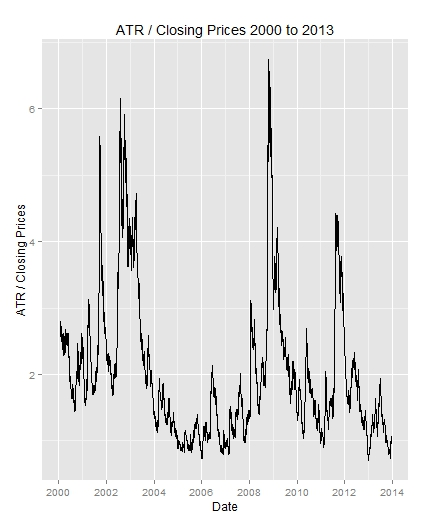
\includegraphics{chp3_Dax_atr}
\caption[ATR of DAX Divided by Closing Price]{ATR of DAX divided by closing price between 2000 and 2013.}
\label{fig:Dax_atr}
\end{figure}

\subsection{Opening Price}
Where a market opens in relation to the previous day's high and low price varies across the data sets. This is important and can influence the technical analysis indicator or trading system to utilise. Table \ref{tab:openprices} lists opening price statistics for a variety of national indices. The table lists the number of times that opening prices are between the previous day's high and low prices. These statistics are useful in characterising a market in terms how they move out of hours and can have an impact when choosing a trading system.

\begin{table}[!htbp] \centering 
  \caption[Opening Prices in relation to previous day's High and Low values]{Opening prices in relation to the previous day's high and low values.} 
  \label{tab:openprices}
\begin{tabular}{lc} 
\toprule 
Market & Opening Price between Previous   \\ 
       &  Day's High and Low (\%) \\
\midrule 
DAX & 75 \\ 
FTSE & 90  \\ 
CAC & 60  \\ 
Dow & 98 \\ 
Nikkei & 53 \\ 
AORD & 79\\ 
\bottomrule 
%\normalsize 
\end{tabular} 
\end{table} 

% Orig table
%\begin{table}[!htbp] \centering 
%  \caption[Opening Prices in relation to previous period.]{Opening prices in relation to the previous day's high and low values a. percentage of times open is between previous high and low b. open price is within a band 10\% below high and above low and c. within a band 30\% below high and above low.} 
%  \label{tab:openprices}
%\begin{tabular}{lccccc} 
%\toprule 
%Market & Open in Prev HL & Open in Prev HL +/-10\% & Open in Prev HL +/-30\%  \\ 
%\midrule 
%DAX & 75\% & 60\% & 29\%  \\ 
%FTSE & 90\% & 70\% & 32\%  \\ 
%CAC & 60\% & 49\% & 25\%  \\ 
%Dow & 98\% & 85\% & 49\%  \\ 
%Nikkei & 53\% & 43\% & 21\%  \\ 
%AORD & 79\% & 64\% & 29\%  \\ 
%\bottomrule 
%%\normalsize 
%\end{tabular} 
%\end{table} 

\subsection{Closing Price}
\label{sec:closing_prices}
In a similar fashion to the opening prices the position of the closing prices in relation to the previous day's high and low price are also of interest. In this case, the percentage of closes outside the previous high / low price may indicate that the market may be a good choice for a breakout type of trading system (see section \ref{sec:chp5:bout_sys} for details of breakout systems). Likewise the opposite situation occurs if a market frequently finishes within the previous day's high and low levels and may be a candidate for a reversal type of system. The statistics for various national indices can be seen in Table \ref{tab:closeHL}. Looking at these figures it would suggest that the Dow with a low ratio of finishing outside the previous period's high low values may be a candidate for a reversal type of system and conversely the Japanese Nikkei has a high percentage value and potentially a candidate for a break-out system.

\begin{table}[!htbp] \centering 
  \caption[Closing Prices in relation to previous day's High and Low values]{Number of occasions when closing prices finished outside the previous day's high or low values.} 
  \label{tab:closeHL}
\begin{tabular}{lc} 
\toprule 
Market & Closing Price outside Previous   \\ 
       &  Day's High and Low (\%) \\
\midrule 
DAX & 56 \\ 
FTSE & 56  \\ 
CAC & 58 \\ 
Dow & 39  \\ 
Nikkei & 63 \\ 
AORD & 60 \\
\bottomrule 
%\normalsize 
\end{tabular} 
\end{table} 

The range from opening price to closing price, either up or down, is of interest. Table \ref{tab:OCrange} lists the minimum and maximum values in this range and Table \ref{tab:OCQuantile} shows the quantiles for this price range.

\begin{table}[!h] \centering 
  \caption[Daily Open to Close Price Range]{Minimum and maximum values for the open to close price range.} 
  \label{tab:OCrange}
\begin{tabular}{lcc} 
\toprule 
Market & Min Value & Max Value  \\ 
\midrule
DAX  & 0 & 508  \\ 
FTSE & 0 & 431  \\ 
CAC  & 0 & 313  \\ 
Dow  & 0 & 950  \\ 
Nikkei & 0 & 1333  \\ 
AORD   & 0 & 347  \\ 
\bottomrule
%\normalsize 
\end{tabular} 
\end{table} 


\begin{table}[!htbp] \centering 
  \caption[Quantiles of the open to close price range]{Quantile values for the open to close price range.} 
  \label{tab:OCQuantile}
\begin{tabular}{lcccc} 
\toprule 
Market & 25\% & 50\% & 75\% & 90\% \\ 
\midrule
DAX  & 16  & 39 & 75 & 508  \\ 
FTSE & 15  & 33 & 63 & 431 \\ 
CAC  & 11  & 26 & 49 & 313 \\ 
Dow  & 27 & 61  & 119 & 950 \\ 
Nikkei & 32  & 71  & 133 & 1333 \\ 
AORD   & 8  & 19  & 36 & 347 \\ 
\bottomrule
%\normalsize 
\end{tabular} 
\end{table} 


%\newcolumntype{d}{D{.}{.}{2.3}}
%\newcolumntype{C}{>{\centering}p}

%\begin{table}[htdp]
%\caption[Closing Prices in relation to previous period.]{Closing prices in relation to the previous day's high and low values.}
%\centering
%\begin{center}
%\begin{tabular}{p{0.7in}ccc}
%\toprule
%\multicolumn{1}{p{0.7in}}{Market} & 
%\multicolumn{1}{C{1.25in}}{Close outside previous HL (\%)} & 
%\multicolumn{1}{C{1.25in}}{Close outside previous HL +/-10\% (\%)} &
%\multicolumn{1}{C{1.25in}}{Close outside previous HL +/-30\% (\%)}\\
%\midrule
%DAX & 56 & 64 & 81  \\ 
%FTSE & 56 & 63 & 81  \\ 
%CAC & 58 & 66 & 83  \\ 
%Dow & 39 & 48 & 72  \\ 
%Nikkei & 63 & 70 & 84  \\ 
%AORD & 60 & 68 & 84  \\ 
%\bottomrule
%\end{tabular}
%\end{center}
%\label{tab:closeHL}
%\end{table}
%
%
%\ctable[
%cap = Closing Prices in relation to previous period,
%caption = Closing prices in relation to the previous day's high and low values
%]
%{lccc }
%{\tnote{Close price is outside of the previous high minus 10\% or the low plus 10\%}
%\tnote[b]{Close price is outside of the previous high minus 30\% or the low plus 30\%}}
%{
%\FL
%Market &  Close Outside   &  Outside Previous      & Outside Previous \\
%DAX    & Previous HL      &  HL +/- 10\% \tmark   &  HL +/- 30\% \tmark[b]         \ML
%DAX & 56 & 64 & 81  \\ 
%FTSE & 56 & 63 & 81  \\ 
%CAC & 58 & 66 & 83  \\ 
%Dow & 39 & 48 & 72  \\ 
%Nikkei & 63 & 70 & 84  \\ 
%AORD & 60 & 68 & 84  \LL
%}


%\begin{table}[!htbp] \centering 
%  \caption[Closing Prices in relation to previous period.]{Closing prices in relation to the previous day's high and low values a. percentage of times close is greater than previous high or lower than previous low b. open price is greater than a band 10\% below high and above low and c. greater than a band 30\% below high and or above the low.} 
%  \label{tab:closeHL2}
%\begin{tabular}{lccccc} 
%\toprule 
%Market & Close out Prev HL & Close out Prev HL(1090) & Close out Prev HL(3070)  \\ 
%\midrule
%DAX & 56\% & 64\% & 81\%  \\ 
%FTSE & 56\% & 63\% & 81\%  \\ 
%CAC & 58\% & 66\% & 83\%  \\ 
%Dow & 39\% & 48\% & 72\%  \\ 
%Nikkei & 63\% & 70\% & 84\%  \\ 
%AORD & 60\% & 68\% & 84\%  \\ 
%{\footnotesize a bit of text} \\
%\bottomrule
%%\normalsize 
%\end{tabular} 
%\end{table} 


\subsection{High / Low Price}
Table \ref{tab:highlow} shows the percentage of times that either today's high price crosses yesterday's high or today's low prices dips below yesterday's low value. The final closing price may be between yesterday's high and low or outside of it. The second column of Table \ref{tab:highlow} is the number of times when today's values crossed both the previous low and the previous high in the same day. This is also known as an Engulfing Candlestick (see section \ref{sec:eng_cand}). In all the indices the previous day's high or low value is reached the following day in a large number of instances, in the case of the Nikkei 90\% of the time. Conversely, the likelihood of both the previous day's high and low values being touched are low, only 5\% of occasions in the Australian AORD. 

\begin{table}[!htbp] \centering 
  \caption[Today's H/L Prices in relation to previous day's HL]{Number of occasions when today's high or low prices crossed the previous day's high or low values.} 
  \label{tab:highlow}
\begin{tabular}{lcc } 
\toprule 
Market & Crosses either previous    & Crosses both the previous \\ 
       & day's High or Low (\%)     &  day's High and Low (\%)       \\
\midrule 
DAX  & 89  & 9  \\ 
FTSE & 87  & 8  \\ 
CAC  & 90  & 10 \\ 
Dow  & 88  & 9  \\ 
Nikkei & 90 & 8 \\ 
AORD   & 86 & 5 \\
\bottomrule 
%\normalsize 
\end{tabular} 
\end{table} 

%\begin{table}[!htbp] \centering 
%  \caption[Today's High/Low Prices in relation to the previous period.]{Today's High/Low prices in relation to the previous day's high and low values a. percentage of times high/low is greater than previous high or lower than previous low b. open price is greater than a band 10\% below high and above low and c. greater than a band 30\% below high and or above the low.} 
%  \label{tab:highlow}
%\begin{tabular}{lcccc} 
%\toprule
%Market & \parbox[c]{2cm}{HL crosses Prev HL} & \parbox[c]{3cm}{HL crosses \\both Prev HL} & \parbox[c]{3cm}{HL crosses\\ Prev HL(1090)} & \parbox[c]{3cm}{HL crosses both Prev HL(1090)}  \\ 
%\midrule
%DAX  & 89\% & 9\%  & 95\% & 16\% \\ 
%FTSE & 87\% & 8\%  & 95\% & 15\% \\ 
%CAC  & 90\% & 10\% & 95\% & 16\% \\ 
%Dow  & 88\% & 9\%  & 97\% & 21\% \\ 
%Nikkei & 90\% & 8\%  & 95\% & 12\% \\ 
%AORD   & 86\% & 5\%  & 94\% & 10\% \\ 
%\bottomrule
%\normalsize 
%\end{tabular} 
%\end{table} 

\subsection{OH/OL Price Fluctuations}
\label{sec:ohol:fluctuation}
The movements in prices between the open and high (OH) and open to low (OL) are interesting and can have an influence on any trading systems developed. On any given day prices open, move to their lowest point, move to their highest point and then close (not in any particular order). From the OHLC data used in this study the order of these events can not be determined or even the number of times in a day these price points are reached. 

In this section we are concerned with the relative sizes of these two price movements, the day's high price minus the opening price (OH) and the opening price minus the low price (OL), one of which is usually greater than the other. We will define the daily \textquotedblleft minor" price fluctuation as the smaller of the two price movements. Likewise we will define the larger value as the \textquotedblleft major" price fluctuation.

Considering the minor price fluctuation, the range of values encountered in the indice markets under study can be seen in Table \ref{tab:minorOH}. In all cases the minimum value is zero, in other words the market opening price and either the day's high or low price were the same, the market didn't dip below or above this level. The second column in Table \ref{tab:minorOH} is the maximum value. In the case of the German DAX, there was a day when the market moved 189 points away from its opening price but also moved further in the opposite direction away from the opening price. Clearly this was a highly volatile day on the German markets.

\begin{table}[!h] \centering 
  \caption[Minor daily price fluctuation]{Minimum and maximum values for the smaller of the daily OH or OL price movement - the \textquotedblleft minor" move.} 
  \label{tab:minorOH}
\begin{tabular}{lcc} 
\toprule 
Market & Min Value & Max Value  \\ 
\midrule
DAX  & 0 & 189  \\ 
FTSE & 0 & 186  \\ 
CAC  & 0 & 134  \\ 
Dow  & 0 & 379  \\ 
Nikkei & 0 & 310  \\ 
AORD   & 0 & 114  \\ 
\bottomrule
%\normalsize 
\end{tabular} 
\end{table} 

The quantiles of the minor price movements can be seen in Table \ref{tab:minorOHQ}. The 90\% quantile is the level at which 90\% of the time the minor move is less than this level.  This value may be important to know and understand when considering break-out type of systems (see section \ref{sec:bout}).  Looking at the value of the DAX we can see that the 90\% quantile level occurs at 46, which indicates that if the market has moved to this level it is unlikely to be the day's minor move (whose level 90\% of the time is below this).  Perhaps a break-out type of system may be profitable at this point, as once the market has moved this far it is usually a major move and may be expected to continue further in the same direction.

\begin{table}[!htbp] \centering 
  \caption[Quantiles of Minor daily price fluctuation.]{Quantile values for the smaller of the days OH or OL price movement - the \textquotedblleft minor" move.} 
  \label{tab:minorOHQ}
\begin{tabular}{lcccc} 
\toprule 
Market & 25\% & 50\% & 75\% & 90\% \\ 
\midrule
DAX  & 5  & 15 & 29 & 46  \\ 
FTSE & 0  & 7 & 20 & 33 \\ 
CAC  & 4  & 11 & 19 & 31 \\ 
Dow  & 12 & 43  & 75 & 113 \\ 
Nikkei & 5  & 21  & 43 & 72 \\ 
AORD   & 0  & 1  & 7 & 13\\ 
\bottomrule
%\normalsize 
\end{tabular} 
\end{table} 

In contrast to the minor daily price fluctuation, the \textquotedblleft major" price fluctuation is defined as the largest of the OH or OL values.  The range of values encountered in this price fluctuation in the indice markets can be seen in Table \ref{tab:majorOH} and the quantiles of the major price movements can be seen in Table \ref{tab:majorOHQ}. Considering the DAX once more, it can be seen that the 25\% quantile is approximately equal to the 90\% quantile of the minor fluctuation. Thus if the DAX moves approximately 50 points away from the opening it is unlikely to be the smaller of the price movements and much more likely to be part of the larger movement. Knowledge of the minor and major price fluctuations may be useful in developing trading systems. 

\begin{table}[!h] \centering 
  \caption[Major daily price fluctuation.]{Minimum and maximum values for the larger of the days OH or OL price movement - the \textquotedblleft major" daily price fluctuation.} 
  \label{tab:majorOH}
\begin{tabular}{lcc} 
\toprule 
Market & Min Value & Max Value  \\ 
\midrule
DAX  & 0 & 530  \\ 
FTSE & 0 & 471  \\ 
CAC  & 0 & 359  \\ 
Dow  & 0 & 992  \\ 
Nikkei & 0 & 1737  \\ 
AORD   & 0 & 347 \\ 
\bottomrule
%\normalsize 
\end{tabular} 
\end{table} 

\begin{table}[!htbp] \centering 
  \caption[Quantiles of Major daily price fluctuation.]{Quantile levels for the larger of the day's OH or OL price movement - the \textquotedblleft major" daily price fluctuation.} 
  \label{tab:majorOHQ}
\begin{tabular}{lccc} 
\toprule 
Market & 25\% & 50\% & 75\% \\ 
\midrule
DAX  & 43  & 69 & 106  \\ 
FTSE & 37  & 56 & 86  \\ 
CAC  & 30  & 45 & 69  \\ 
Dow  & 92 & 131  & 190  \\ 
Nikkei & 76  & 118  & 184  \\ 
AORD   & 18  & 30  & 48 \\ 
\bottomrule
%\normalsize 
\end{tabular} 
\end{table} 

A final consideration in this section is the range of the open to close prices detailed in section \ref{sec:closing_prices}. Again considering the German DAX it can be seen that the 50\% quantile value is 39, as shown in Table \ref{tab:OCQuantile}, which is below the 90\% minor fluctuation level.

%\begin{table}[!htbp] \centering 
%  \caption[Quantiles of the open to close price range.]{Quantile values for the open to close price range.} 
%  \label{tab:OCQuantile2}
%\begin{tabular}{lcccc} 
%\toprule 
%Market & 25\% & 50\% & 75\% & 90\% \\ 
%\midrule
%Dax  & 16  & 39 & 75 & 508  \\ 
%FTSE & 15  & 33 & 63 & 431 \\ 
%CAC  & 11  & 26 & 49 & 313 \\ 
%Dow  & 27 & 61  & 119 & 950 \\ 
%Nikkei & 32  & 71  & 133 & 1333 \\ 
%AORD   & 8  & 19  & 36 & 347 \\ 
%\bottomrule
%%\normalsize 
%\end{tabular} 
%\end{table} 

\section{Software Tools}

\subsection{R and R Studio}
Experimental results and graphs were produced with the open source programming language R version 3.0.2. For help in the creation and organisation of the R code for this thesis the open-source development environment R Studio version 0.98.490 was used extensively. The following packages were immensely helpful in the preparation of this thesis:
\begin{itemize}
\item TTR - provided technical analysis functions
\item xts - irregularly spaced time series
\item forecast - time series forecasting
\item candlestick - Japanese candlestick patterns
\end{itemize}

\subsection{Rapid Miner}
Rapid Miner version 5.3, a market leading open-source data mining and predictive analytic platform, was used for building hybrid ARIMA models. The base system and time series plug-ins were used.

\section{Methodology}
The aim of this study was to predict market movement, not in terms of absolute values but  more in terms of general direction. The trading algorithms developed in this study were based around a daily time period. The data used was daily data containing open, high, low and closing prices. The trading algorithms developed typically opened a trade at the day's opening price and closed them at the day's closing prices. There are some deviations from this, for example trades are closed at some pre-defined point in the event of a stop loss being entered or trades running from close to close, and these are detailed in the text at the appropriate place. The forecasts produced from the technical analysis and time series models were consumed by the trading algorithms and used to decide in which direction the daily trade would be made, i.e. would the market rise or fall.

The success or failure of any particular method was determined by the number of points gained or lost in these trading algorithms. In turn these points can be considered money and the net number of points can represent a profit or loss (PL). The results presented in Chapters \ref{Chapter4} and \ref{Chapter5} report either the total PL of a system or the average PL per trade. The latter value is probably most useful when it comes to comparing systems that don't enter trades every day, for example when one uses candlestick patterns which only occur very infrequently. Also the direction of trade is also a consideration. Results are separated into long (a buy is made in the expectation of the market rising) or short (a sell is made in the expectation of the market falling).
